
\chapter{Soluzione proposta}
Come evidenziato dalla traccia ci sono alcune frasi da tradurre. Quindi come prima cosa si è cercato di fare luce sui vari step da intraprendere per lo svolgimento del progetto.\\
Essenzialmente sono stati individuati 3 step fondamentali:
\begin{itemize}
	\item \textbf{Step 1}: Parsing;
	\item \textbf{Step 2}: Elaborazione PoS e Sentence Plan;
	\item \textbf{Step 3}: Traduzione e generazione della frase.
\end{itemize}
\textbf{Step 1}\\
Per prima cosa si è scelto di utilizzare \textbf{Tint} per effettuare il parsing delle frasi fornite, le quali sono:
\begin{itemize}
	\item È la spada laser di tuo padre;
	\item Ha fatto una mossa leale;
	\item Gli ultimi avanzi della vecchia Repubblica sono stati spazzati via.
\end{itemize}
L'operazione di parsing produce un Json in cui sono annotate le dipendenze che si trovano all'interno della frase analizzata con gli opportuni riferimenti. Ad esempio, per una certa parola analizzata viene specificato il suo "index", ovvero la posizione che essa occupa nella frase. Inoltre ci sono altre informazioni importanti per il prosieguo del progetto come la dipendenza che la parola rappresenta e soprattutto i Governor e Dependent. I suoi campi sono:
\begin{itemize}
	\item \textbf{dep}: tipologia dipendenza.
	\item \textbf{governorGloss}: head della dipendenza.
	\item \textbf{dependentGloss}: dependent della dipendenza.
\end{itemize}
Le dipendenze vengono poi sfruttate per la costruzione della struttura sintattica ad albero su cui lavorare. Un altro aspetto molto importante riguarda le feature linguistiche fornite da Tint stesso: quelle relative alle forme verbali permetteranno poi il corretto settaggio dei metodi per l'impostazione del tempo verbale all'interno della frase.\\
Un altro strumento che Tint mette a disposizione è la visualizzazione grafica degli alberi generati: 
\begin{figure}[h!]
	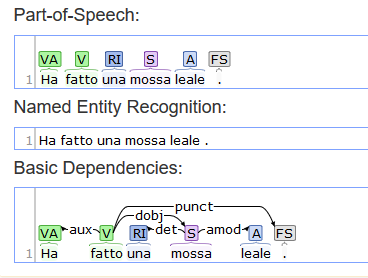
\includegraphics[scale=0.65]{F1.png}
	\centering
	\label{fig:ACT}
\end{figure}
\begin{figure}[h!]
	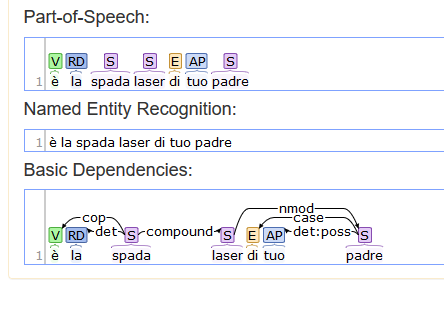
\includegraphics[scale=0.65]{F2.png}
	\centering
	\label{fig:ACT}
\end{figure}
\clearpage
\begin{figure}[h!]
	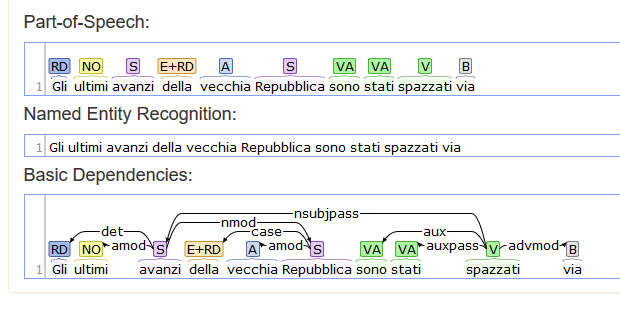
\includegraphics[scale=0.65]{F3.png}
	\centering
	\caption{Alberi a dipendenze delle frasi analizzate.}
	\label{fig:ACT}
\end{figure}
Attraverso queste rappresentazioni è stato possibile effettuare il mapping tra le dipendenze e la struttura di SimpleNLG. Inoltre, sono state molto utili per capire come muoversi nella costruzione della frase.\\
\textbf{Step 2}\\
Una volta ottenute le informazioni necessarie dalla fase precedente è possibile passare alla creazione del Sentence Plan. In questo caso abbiamo utilizzato solo alcune delle info elaborate, come ad esempio il PoS, la stringa elaborata e la feature (ad esempio, per un verbo il tempo di coniugazione); a questo si aggiunge un ID andando a formare una quadrupla che identifica la parola nel Sentence Plan.\\
Grazie al mapping tra le dipendenze di Tint e la struttura di SimpleNLG si possono implementare dei controlli attraverso cui analizzare l'albero generato e in seguito impostare i parametri del Sentence Plan stesso.\\
\textbf{Step 3}\\
Una volta impostata quindi la costruzione della frase, si passa alla traduzione dei vari lessemi. Si è realizzato un piccolo dizionario in cui sono presenti le parole contenute nelle frasi, con l'aggiunta di altre affini. Effettuata quindi la traduzione, si passa alla fase di generazione e successivamente all'output.
\clearpage

\section{Risorse utilizzate}
\subsection{Tint (The Italian NLP Tool)}
Tale strumento è una pipeline per \textbf{Natural Language Processing (NLP)} in italiano. È molto veloce e preciso e implementa la maggior parte degli strumenti linguistici comuni, come la codifica delle parti del discorso e l'analisi delle dipendenze. Lo strumento è basato su Stanford CoreNLP e può essere utilizzato come strumento autonomo, includendo le dipendenze in  Java all'interno del file "pom.xml".\\
\subsection{SimpleNLG}
SimpleNLG è una liberia Java che permette di eseguire attività semplici, utili e necessarie per la generazione del linguaggio naturale (NLG). La libreria è stata utile in quanto, grazie ad essa, si sono creati i metodi per la costruzione, seguita poi dalla generazione della frase.\\
Le classi utilizzate permettono inoltre di specificare le componenti della frase (Soggetto, Verbo, Complemento Oggetto) e anche complementi aggiuntivi (Aggettivi, Avverbi).



